\documentclass[12pt]{article}


\usepackage{amssymb}
\usepackage{amsmath}
\usepackage{fullpage}
\usepackage{epsfig}
\usepackage{epstopdf}
\everymath{\displaystyle}



\begin{document}

\begin{center}
\underline{\LARGE{Chapter 4.8 Practice Problems}}
\end{center}

\noindent EXPECTED SKILLS:

\begin{itemize}

\item Understand the hypotheses and conclusion of Rolle's Theorem or the Mean Value Theorem.

\item Be able to find the value(s) of ``$c$" which satisfy the conclusion of Rolle's Theorem or the Mean Value Theorem.

\end{itemize}

\noindent PRACTICE PROBLEMS:

\medskip

\begin{enumerate}

\item For each of the following, verify that the hypotheses of Rolle's Theorem are satisfied on the given interval. Then find all value(s) of $c$ in that interval that satisfy the conclusion of the theorem.

\begin{enumerate}

\item $f(x)=x^2-4x-11$; $[0,4]$

\includegraphics[scale=0.5]{start.pdf}
{{{1\linewidth}{$f(x)$ is a polynomial; so, it is continuous and differentiable everywhere on $(-\infty,\infty)$.  In particular, it is continuous on $[0,4]$ and differentiable on $(0,4)$.  Finally, notice that $f(0)=f(4)=-11$.  Thus, all of the hypotheses of Rolle's Theorem are satisfied and there exists a $c$ in $(0,4)$ with $f^{\prime}(c)=0$.  In particular, $c=2$.}}}
\includegraphics[scale=0.5]{end.pdf}


\item $f(x)=\sin{x}$; $[0,2\pi]$

\includegraphics[scale=0.5]{start.pdf}
{{{1\linewidth}{$f(x)$ is continuous and differentiable everywhere on $(-\infty,\infty)$.  In particular, it is continuous on $[0,2\pi]$ and differentiable on $(0,2\pi)$.  Finally, notice that $f(0)=f(2\pi)=0$.  Thus, all of the hypotheses of Rolle's Theorem are satisfied and there exists a $c$ in $(0,2\pi)$ with $f^{\prime}(c)=0$.  In particular, $c$ is either $\frac{\pi}{2}$ or $\frac{3\pi}{2}$.}}}
\includegraphics[scale=0.5]{end.pdf}


\end{enumerate}

\item Let $f(x)=\frac{1}{x^2}$

\begin{enumerate}

\item Show that there is no point $c$ in the interval $(-1,1)$ such that $f^{\prime}(c)=0$, even though $f(-1)=f(1)=1$.

\includegraphics[scale=0.5]{start.pdf}
{{{1\linewidth}{$f^{\prime}(x)=-\frac{2}{x^3}$ which is never 0.  Thus, there does not exist a $c$ in $(-1,1)$ with $f^{\prime}(c)=0$.}}}
\includegraphics[scale=0.5]{end.pdf}


\item Explain why the result from part (a) does not contradict Rolle's Theorem.

\includegraphics[scale=0.5]{start.pdf}
{{{1\linewidth}{$f(x)$ is not continuous at $x=0$ which is in $[-1,1]$, so Rolle's Theorem doesn't apply.}} }
\includegraphics[scale=0.5]{end.pdf}


\end{enumerate}

\item For each of the following, verify that the hypotheses of the Mean Value Theorem are satisfied on the given interval. Then find all value(s) of $c$ in that interval that satisfy the conclusion of the theorem.

\begin{enumerate}

\item $f(x)=x^2-4x$; $[1,5]$

\includegraphics[scale=0.5]{start.pdf}
{{{1\linewidth}{$f(x)$ is a polynomial; so, it is continuous and differentiable everywhere on $(-\infty,\infty)$.  In particular, it is continuous on $[1,5]$ and differentiable on $(1,5)$.  Thus, all of the hypotheses of the Mean Value Theorem are satisfied and there exists a $c$ in $(1,5)$ with $f^{\prime}(c)=\frac{f(5)-f(1)}{5-1}$.  In particular, $c=3$.}}}
\includegraphics[scale=0.5]{end.pdf}


\item $f(x)=x-\cos{x}$; $[0,2\pi]$

\includegraphics[scale=0.5]{start.pdf}
{{{1\linewidth}{$x$ is a polynomial and is, therefore, continuous and differentiable everywhere on $(-\infty,\infty)$.  $\cos{x}$ is also continuous and differentiable everywhere on $(-\infty,\infty)$.  So, since the difference of continuous functions is continuous and the difference of differentiable functions is differentiable, we have that $f(x)$  is continuous and differentiable everywhere on $(-\infty,\infty)$.  In particular, it is continuous on $[0,2\pi]$ and differentiable on $(0,2\pi)$.  Thus, all of the hypotheses of the Mean Value Theorem are satisfied and there exists a $c$ in $(0,2\pi)$ with $f^{\prime}(c)=\frac{f(2\pi)-f(0)}{2\pi-0}$.  In particular, $c=\pi$.}}}
\includegraphics[scale=0.5]{end.pdf}


\end{enumerate}

\item Let $f(x)=x^{2/3}$

\begin{enumerate}

\item Show that there is no point $c$ in $(-8,1)$ such that $f^{\prime}(c)$ will be equal to the slope of the secant line through $(-8,f(-8))$ and $(1,f(1))$.

\includegraphics[scale=0.5]{start.pdf}
{{{1\linewidth}{It can be shown that the slope of the secant line which passes through $(-8,f(-8))$ and $(1,f(1))$ is $-\frac{1}{3}$.  And, $f^{\prime}(x)=\frac{2}{3x^{1/3}}$.  However, the only solution to $f^{\prime}(x)=-\frac{1}{3}$ is $-8$, which is not in $(-8,1)$.}}}
\includegraphics[scale=0.5]{end.pdf}


\item Explain why the result from part (a) does not contradict the Mean Value Theorem.

\includegraphics[scale=0.5]{start.pdf}
{{{1\linewidth}{$f(x)$ is not differentiable at $x=0$ which is in $(-8,1)$.  Thus, the Mean Value Theorem does not apply.}}}
\includegraphics[scale=0.5]{end.pdf}


\end{enumerate}

\newpage

\item Consider $f(x)=x^3-x^2$.

\begin{enumerate}

\item Find the value(s) of $c$ which satisfy the conclusion of the Mean Value Theorem on $[-4,4]$.

\includegraphics[scale=0.5]{start.pdf}
{{$c=-2$ or $c=\frac{8}{3}$}}
\includegraphics[scale=0.5]{end.pdf}


\item At each value of $c$ found in part (a), calculate an equation of the line which is tangent to the graph of $f(x)$.

\includegraphics[scale=0.5]{start.pdf}
{{$y=16x-20$; $y=16x-\frac{832}{27}$}}
\includegraphics[scale=0.5]{end.pdf}


\item On the axes provided below, sketch the tangent lines which you found in part (b).

\begin{center}
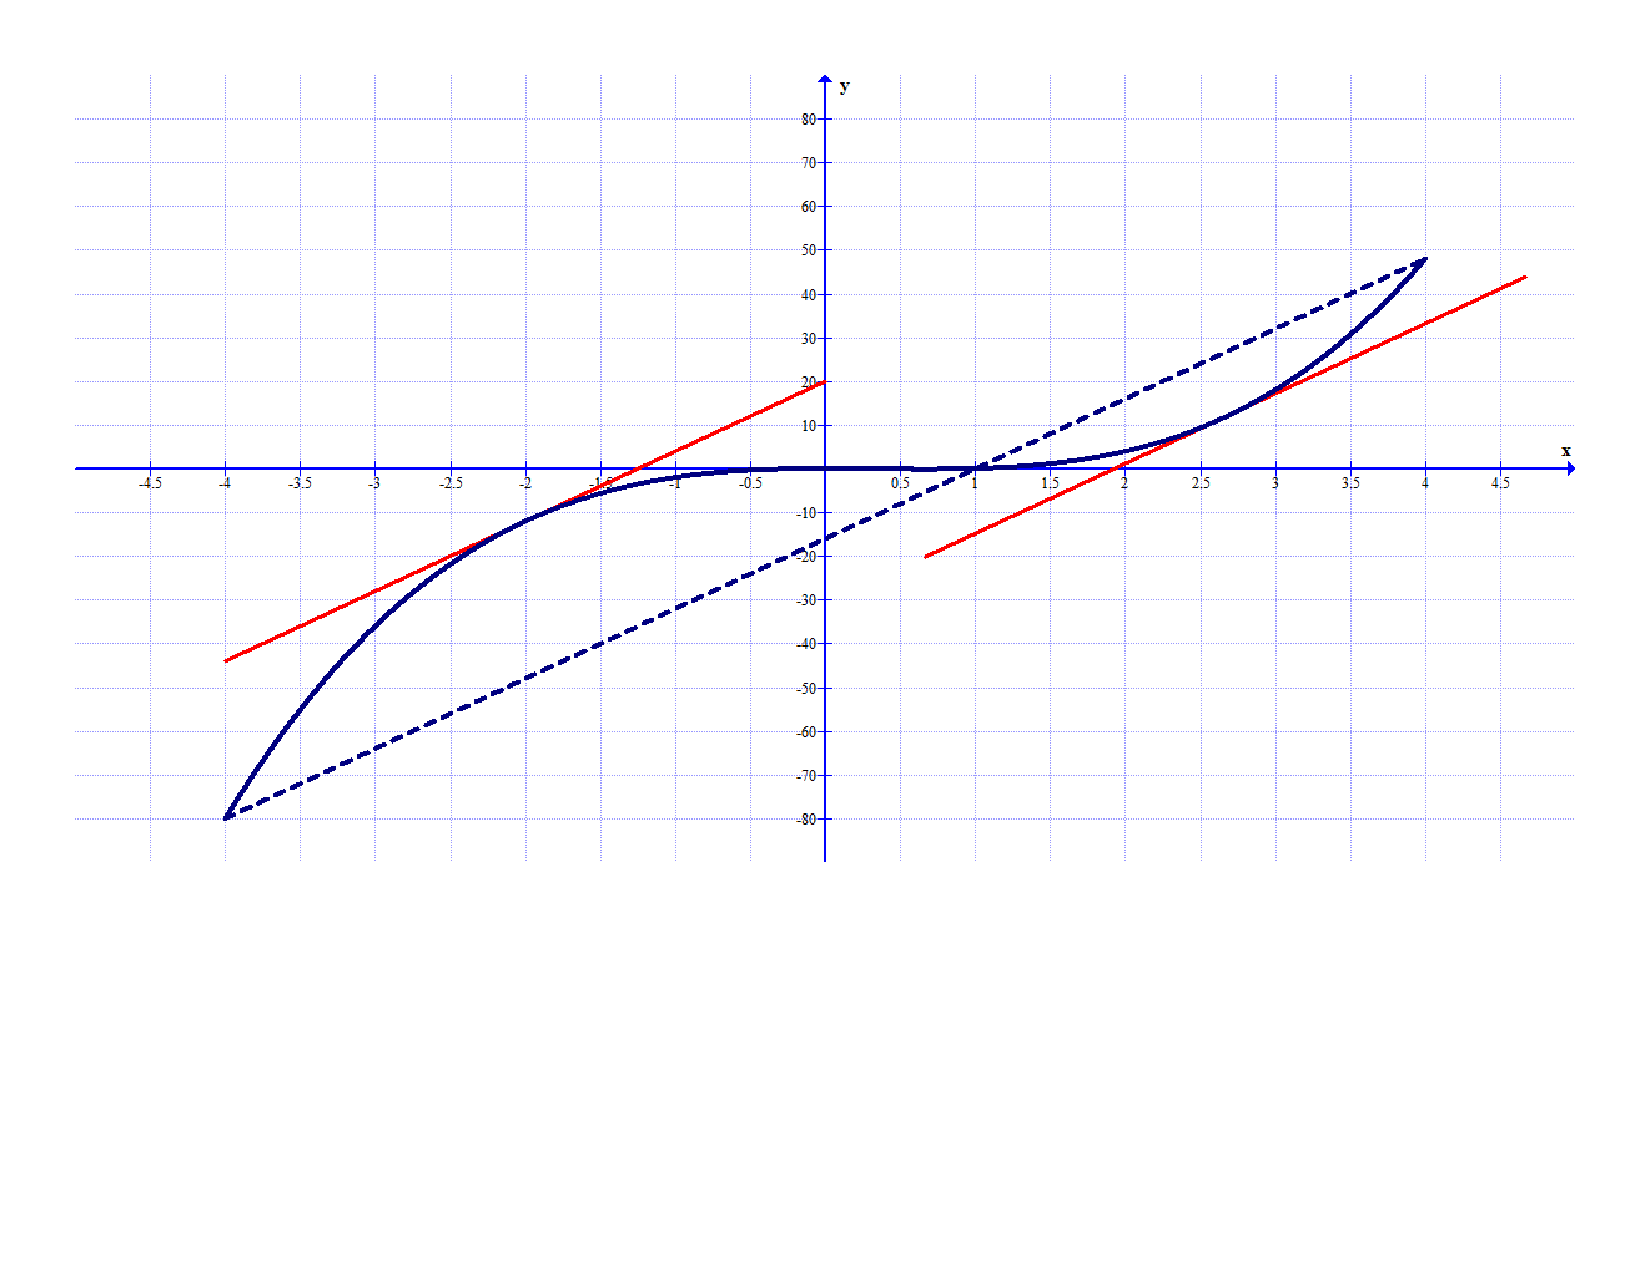
\includegraphics[scale=0.4]{grapha.pdf}
\end{center}

\end{enumerate}

\item Consider the quadratic function $f(x)=c_1x^2+c_2x+c_3$, where $c_1 \neq 0$.  Show that the number $c$ in the conclusion of the mean value theorem is always the midpoint of the given interval $[a,b]$.

\includegraphics[scale=0.5]{start.pdf}
{{{1\linewidth}{Since $f(x)$ is a polynomial, it is continuous and differentiable everywhere on $(-\infty,\infty)$.  In particular, it is continuous on $[a,b]$ and differentiable on $(a,b)$.  Thus, there is a $c$ in $(a,b)$ such that $f^{\prime}(c)=\frac{f(b)-f(a)}{b-a}$.

Notice that:
\begin{align*}
\frac{f(b)-f(a)}{b-a}&=\frac{(c_1b^2+c_2b+c_3)-(c_1a^2+c_2a+c_3)}{b-a}\\
&=\frac{c_1(b^2-a^2)+c_2(b-a)}{b-a}\\
&=c_1(b+a)+c_2
\end{align*}

Finally, notice that $f^{\prime}(x)=2c_1x+c_2$.  Setting this equal to $c_1(b+a)+c_2$ and solving for $x$ yields $x=\frac{b+a}{2}$.  Thus, the value of $c$ in the conclusion of the MVT is $c=\frac{b+a}{2}$, which is the midpoint of the interval $[a,b]$}}}
\includegraphics[scale=0.5]{end.pdf}


\item {\bf Theorem:} Suppose that $f^{\prime}(x)=0$ for all $x$ in some open interval $I$.  Then, $f(x)$ is constant on the interval.

Prove this theorem. (HINT: Consider any two numbers $a$ and $b$ in the interval $I$, where $a<b$.  Show that $f(a)=f(b)$ on the interval $I$.)

\includegraphics[scale=0.5]{start.pdf}
{{{1\linewidth}{Pick any two numbers $a$ and $b$ in the interval $I$, where $a<b$.  Since, by assumption,  $f(x)$ is differentiable for all $x$ in $I$, we have the following:
\begin{itemize}
\item $f(x)$ is continuous on $[a,b]$
\item $f(x)$ is differentiable on $(a,b)$
\end{itemize}
Therefore, by the Mean Value Theorem, there exists a number $c$ in $(a,b)$ such that $$f^{\prime}(c)=\frac{f(b)-f(a)}{b-a}$$  But, $f^{\prime}(x)=0$ for all x in the interval $I$; so, in particular, $f^{\prime}(c)=0$.  Thus, it follows that $f(b)-f(a)=0 \implies f(b)=f(a)$.  In other words, $f(x)$ is constant on the interval $I$.}}}
\includegraphics[scale=0.5]{end.pdf}


\item {\bf Definition:} A function $F(x)$ is an \underline{antiderivative} of $f(x)$ if $\frac{d}{dx}\left[F(x)\right]=f(x)$.  For example, since $\frac{d}{dx}\left[x^2+6\right]=2x$, we say that $F(x)=x^2+6$ is an antiderivative of $f(x)=2x$.

\begin{enumerate}

\item List some other antiderivatives of $2x$.

\includegraphics[scale=0.5]{start.pdf}
{{All antiderivatives of $2x$ have the form $x^2+C$, where $C$ is any constant.}}
\includegraphics[scale=0.5]{end.pdf}


\item {\bf Theorem:} Suppose $g^{\prime}(x)=f^{\prime}(x)$ for all $x$ in an open interval $I$.  Then, for some constant $c$, $g(x)=f(x)+c$ for all $x$ in the interval $I$.

Prove this theorem.  (HINT: Define a new function $h(x)=g(x)-f(x)$ and appeal to the theorem in problem 7.)

\includegraphics[scale=0.5]{start.pdf}
{{{1\linewidth}{Define $h(x)=g(x)-f(x)$.  Then, for all $x$ in the interval $I$,
$$h^{\prime}(x)=g^{\prime}(x)-f^{\prime}(x)=0$$
By problem 7, we know that $h(x)=C$ for some constant $C$. And, it follows that $g(x)=f(x)+C$.
}}}
\includegraphics[scale=0.5]{end.pdf}


\newpage

\item Let $f(x)=\sin^{-1}(x)$ and $g(x)=-\cos^{-1}(x)$.  Verify that $f^{\prime}(x)=g^{\prime}(x)$ and find the constant $C$ such that $\sin^{-1}(x)=-\cos^{-1}(x)+C$.

\includegraphics[scale=0.5]{start.pdf}
{{{1\linewidth}{\begin{center}$f^{\prime}(x)=g^{\prime}(x)=\frac{1}{\sqrt{1-x^2}}$\\
$\sin^{-1}(x)=-\cos^{-1}(x)+\frac{\pi}{2}$ for all $x$ in $[-1,1]$
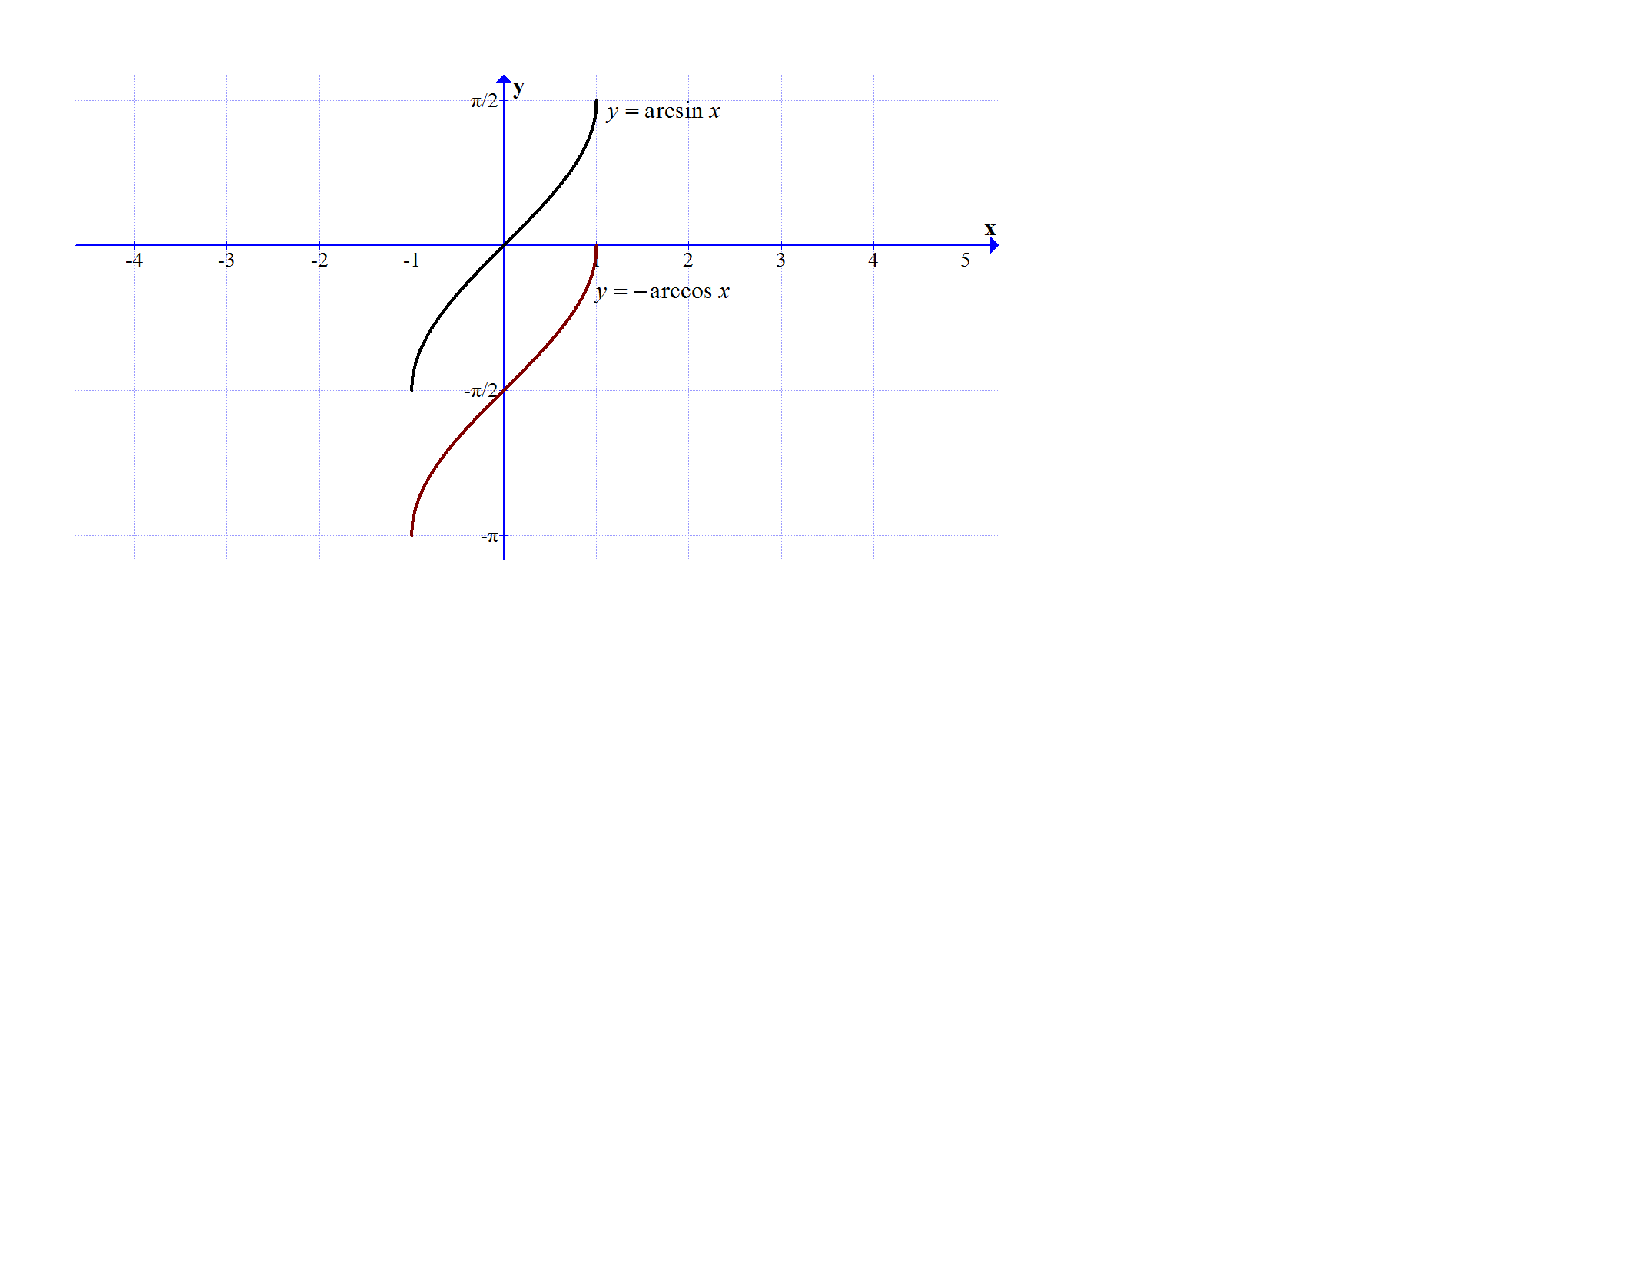
\includegraphics[scale=0.5]{antiderivative.pdf}
\end{center}}}}
\includegraphics[scale=0.5]{end.pdf}


\end{enumerate}

\end{enumerate}

\end{document}